\documentclass[unicode, notheorems]{beamer}

% If you have more than three sections or more than three subsections in at least one section,
% you might want to use the [compress] switch. In this case, only the current (sub-) section
% is displayed in the header and not the full overview.
\mode<presentation>
{
  \usetheme[numbers, totalnumbers, minimal]{Statmod}

  \setbeamercovered{transparent}
  % or whatever (possibly just delete it)
}

%\usepackage{pscyr}
\usepackage[T2A]{fontenc}
\usepackage[utf8]{inputenc}
\usepackage[russian]{babel}
\usepackage{amsthm}

\usepackage{graphicx}
\graphicspath{ {media/} }


%\usepackage{tikz}
% you only need this when using TikZ graphics

\newtheorem{theorem}{Теорема}
\newtheorem{example}{Пример}
\newtheorem{definition}{Определение}

\title{Устранение экспоненциальной сложности оценки стоимости бермудского опциона}

\author{Анастасия Миллер}
\institute[СПбГУ]{Санкт-Петербургский государственный университет \\
    Математико-механический факультет \\
    Кафедра статистического моделирования \\
    \vspace{0.4cm}
    Научный руководитель: д.ф.-м.н. Ермаков С.М. \\
    \vspace{0.3cm}
}
\date{
    Санкт-Петербург\\
    \today
}

% \subject{Beamer}
% This is only inserted into the PDF information catalog. Can be left
% out.

% Delete this, if you do not want the table of contents to pop up at
% the beginning of each subsection:
% \AtBeginSubsection[]
% {
%   \begin{frame}<beamer>
%     \frametitle{Outline}
%     \tableofcontents[currentsection,currentsubsection]
%   \end{frame}
% }

\begin{document}

\begin{frame}
    \titlepage
\end{frame}

\section{Вступление}

  \begin{frame}
    \frametitle{Основные понятия}

    \begin{definition}
      \emph{Опцион} -- договор, по которому потенциальный покупатель или потенциальный продавец актива (товара, ценной бумаги) получает право, но не обязательство, совершить покупку или продажу данного актива по заранее оговорённой цене в определённый договором момент в будущем или на протяжении определённого отрезка времени.
    \end{definition}
  \end{frame}

  \begin{frame}
    \frametitle{Основные понятия}

    \begin{block}{}
    Справедливой ценой опциона будет максимальная выручка, которую можно получить от исполнения опциона.
    \end{block}
    Дискретные оценки: состояние актива меняется только в определённых точках, этих точек конечное число.
    
  \end{frame}

\section{Алгоритм}

  \begin{frame}
    \frametitle{Броуди-Глассерман}
    \begin{figure}[h]
      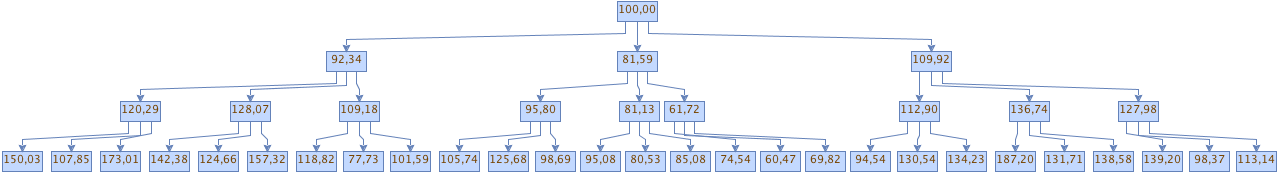
\includegraphics[width=\textwidth]{exp_tree}
      \caption{Дерево, генерируемое при использовании метода, описываемого Глассерманом (цифры в узлах -- стоимость актива)}
      \label{fig:exponentialTree}
    \end{figure}
    Количество узлов в дереве растёт экспоненциально
  \end{frame}

  \begin{frame}
    \frametitle{Решение}
    \onslide<1>
    \alert{Что делать?} 
    \onslide<2->
    Выкидывать вершины из дерева
    \onslide<3>
      \begin{figure}[h]
        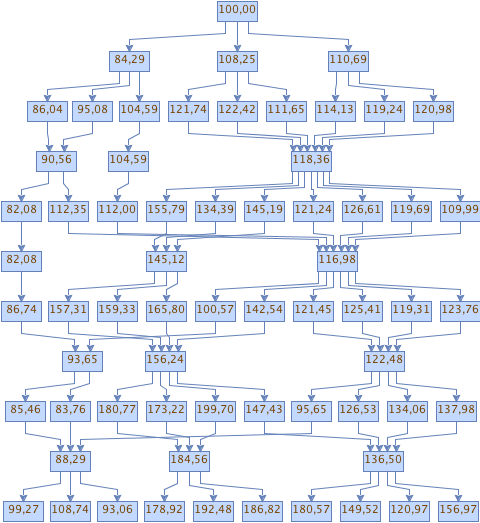
\includegraphics[height=0.5\paperheight]{linear_tree}
        \caption{Дерево, генерируемое усечённым методом (цифры -- стоимость актива; ширина дерева $n=10$, количество секторов $k=3$)}
        \label{fig:linearTree}
      \end{figure} 
  \end{frame}

  \begin{frame}
    \frametitle{Решение}
    \onslide<1>
    \alert{Как делать?} 
    \onslide<2->
    На Java, объектами.
    \onslide<3-> 
    \begin{enumerate}
      \item Реализовать исходные деревья
      \item Реализовать оценки
      \item Реализовать усечённые деревья
      \item Применить к ним оценки
      \item Посмотреть, не стало ли сильно хуже
    \end{enumerate}
  \end{frame}

  \begin{frame}
    \frametitle{Детали}
    \alert{Как усекать деревья?}
    \onslide<2->
    Смотрим на последний ряд дерева
    \onslide+<2->
    \begin{figure}[h]
      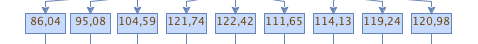
\includegraphics[width=0.8\linewidth]{tree_row}
      \label{fig:linearTree}
    \end{figure}
    \onslide<3->
    $\min = 86.04, \max = 122.98$ \\
    $\frac{\max - \min}{3} = 12.31$ -- величина сектора\\
    \onslide<4>
    Сектора: $[86.04;98.35]\quad[98.35;110.66]\quad[110.66;122.98]$

  \end{frame}

  \begin{frame}
    \frametitle{Детали}
    \alert{Как усекать деревья?}
    Смотрим на последний ряд дерева
    \begin{figure}[h]
      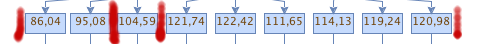
\includegraphics[width=0.8\linewidth]{tree_row_sectorized}
    \end{figure}
    $\min = 86.04, \max = 122.98$ \\
    $\frac{\max - \min}{3} = 12.31$ -- величина сектора\\
    Сектора: $[86.04;98.35]\quad[98.35;110.66]\quad[110.66;122.98]$

  \end{frame}
  
  \begin{frame}
    \frametitle{Детали}
    Считаем средние арифметические по секторам
    \begin{figure}[h]
      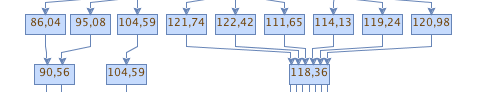
\includegraphics[width=0.8\linewidth]{tree_row_means}
    \end{figure}
  \end{frame}
  
  \begin{frame}
    \frametitle{Детали}
    Рожаем новый ряд от средних арифметических (в соответствии с весами)
    \begin{figure}[h]
      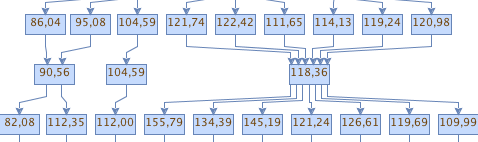
\includegraphics[width=0.8\linewidth]{tree_row_new_generation}
    \end{figure}
    \onslide<2->
    ...и повторяем до достижения нужного числа рядов
  \end{frame}

  \begin{frame}
    \frametitle{Решение}
    Каждый ряд соответствует дате исполнения опциона. Всего дат $s$. При $s\to\infty$ получаем американский опцион.
      \begin{figure}[h]
        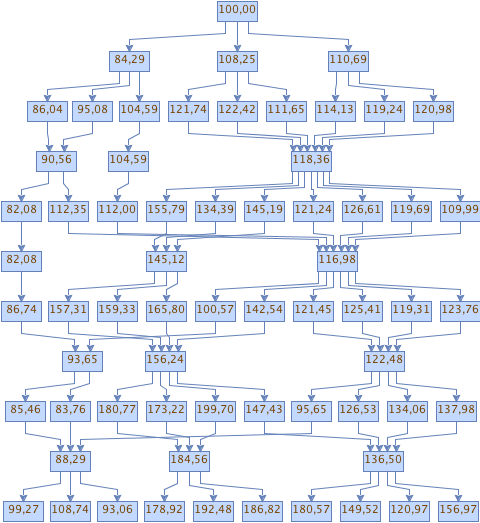
\includegraphics[height=0.5\paperheight]{linear_tree}
        \caption{Дерево, генерируемое усечённым методом (цифры -- стоимость актива; ширина дерева $n=10$, количество секторов $k=3$)}
      \end{figure} 
  \end{frame}

\section{Результаты}
  \begin{frame}
    \frametitle{Сходимость верхней оценки}
      \begin{figure}[h]
        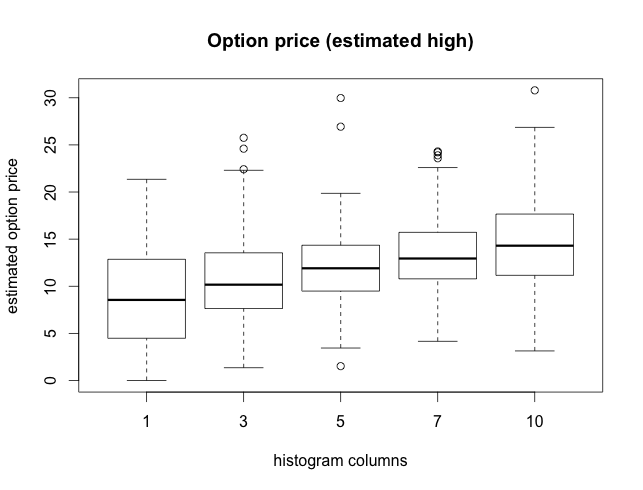
\includegraphics[width=\linewidth, height=0.8\paperheight]{upper_estimate}
      \end{figure} 
  \end{frame}

  \begin{frame}
    \frametitle{Сходимость нижней оценки}
      \begin{figure}[h]
        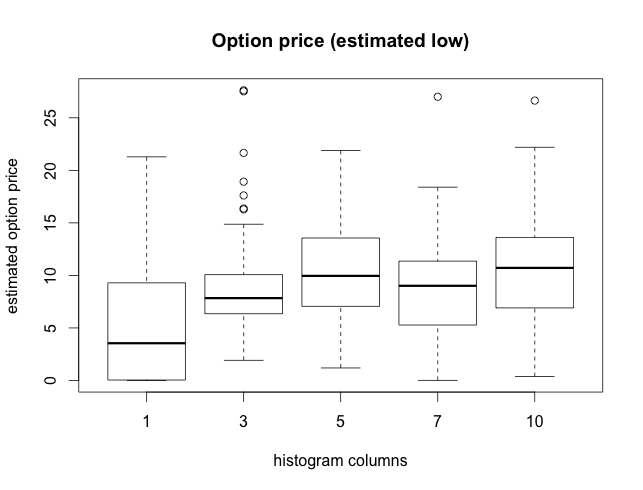
\includegraphics[width=\linewidth, height=0.8\paperheight]{lower_estimate}
      \end{figure} 
  \end{frame}

  \begin{frame}
    \frametitle{Планы}
    \begin{enumerate}
    \item Закончить рассмотрение оценки по гистограмме, в т.ч.\ найти аналитически математическое ожидание оценки
    \item Рассмотреть оценку по кластерам
    \item Рассмотреть другие оценки
  \end{enumerate} 
  \end{frame}

\end{document}
